\documentclass[a4paper, 12pt]{article}
\usepackage[T1]{fontenc}
\usepackage[utf8]{inputenc}
\usepackage{booktabs}
\usepackage{titling}
\usepackage{titlesec}
\usepackage{amssymb}
\usepackage{pifont}
\usepackage{graphicx}
\graphicspath{ {../../} }

\usepackage{hyperref}
\hypersetup{
    colorlinks=true,
    linkcolor=black,
    urlcolor=cyan,
}
\urlstyle{same}

\renewcommand{\contentsname}{Obsah}
\renewcommand{\thesection}{\Roman{section}}
\renewcommand{\thesubsection}{\roman{subsection}}
\renewcommand{\thesubsubsection}{\roman{subsection}.\roman{subsubsection}}

\titleformat{\section}
{\Large\bfseries}
{\thesection}
{0.5em}
{}


\titleformat{\subsection}
{\large\bfseries}
{\thesubsection.}
{0.5em}
{}

\titleformat{\subsubsection}
{\large\bfseries}
{\thesubsubsection}
{0.5em}
{}

\title{
        \vspace{1in}
        \rule{\linewidth}{0.5pt}
		\usefont{OT1}{bch}{b}{n}
        \huge Programátorská dokumentace \\GrainSim\\
        \vspace{-10pt}
        \rule{\linewidth}{1pt}
}
\author{
		\normalfont\normalsize
        Marek Bečvář\\[-3pt]\normalsize
        31.7.2021
}
\date{}


\begin{document}
\maketitle 
\newpage

\tableofcontents
\newpage

\section{Rozbor specifikací} 
\subsection{Popis}
\paragraph{} 
Projekt GrainSim měl za cíl vytvořit v jazyce C\# a frameworku Monogame 2D
herní prostředí, ve kterém si uživatel bude moci tvořit experimenty s látkami, 
jejichž vlastnosti budou založené na těch reálných. V prostředí pak mohou
látky jak navzájem, tak v reakci na prostředí reagovat (výbušniny, hořlaviny,
přeměny skupenství, atd.).

\subsection{Funkční požadavky}
\emph{(z finální verze specifikace zápočtového projektu)}\\
\\
Na základě uživatelem vložených prvků aplikace:
\vspace{-5px}
\begin{itemize}
    \item vykresluje aktuální mapu prostředí 
    \item očekává další vstup od uživatele (výběr jiného prvku, změna
        vykreslovací mapy, aj.)
    \item v každém kroku simulace:
        \begin{itemize}
            \item přesouvá podle daných pravidel prvky po prostředí
            \item přepočítává teplotní mapu prostředí
            \item kontroluje prvky na možné reakce (na základě okolních prvků a
            teplot)
        \end{itemize}
\end{itemize}

\newpage
\section{Architektura/Design}
\small{\emph{Architektura programu byla před zahájením projektu načtrtnuta do
        UML grafu (které se v průběhu práce na projektu někdy rozrostlo, ale 
        velké změny nikdy nenastaly). To co si určitě z tohoto kurzu odnesu dál 
        je síla takového náčrtu, kdy člověk dokáže vyřešit problémy v architektuře 
daleko dříve, než se k nim vlastně dostane.}}

\begin{center}
    \hspace*{-80px}
    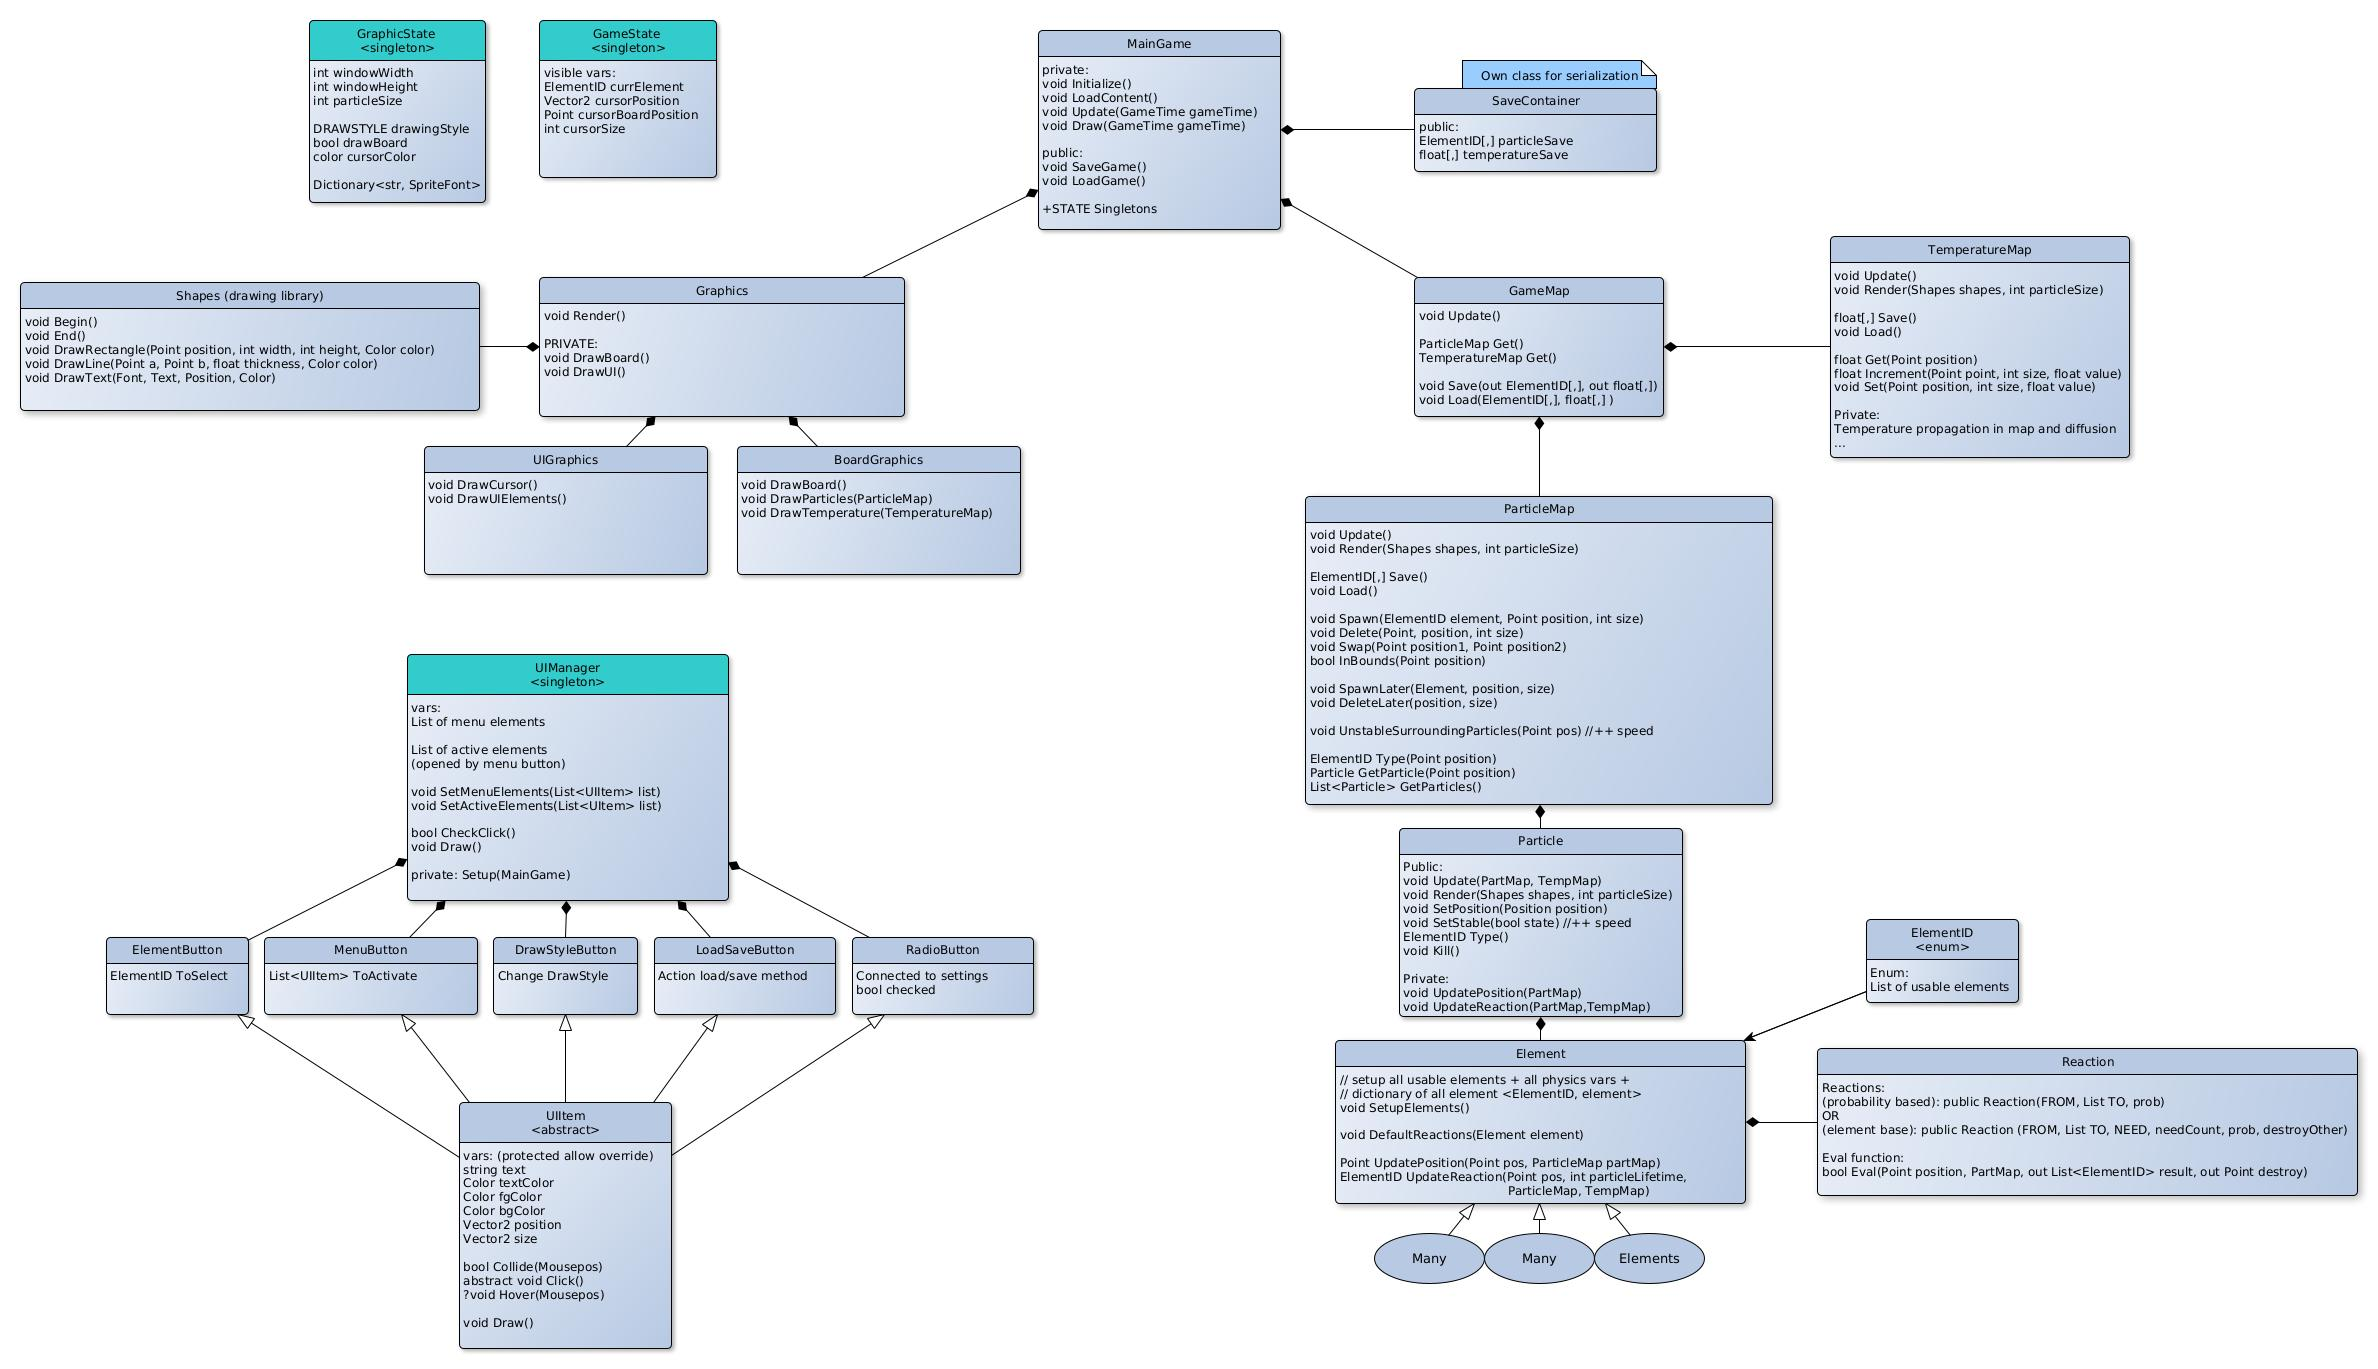
\includegraphics[width=1.4\linewidth]{GrainSim-graph.jpg}
\end{center}

\paragraph{Rozdělení}
Celý program se dělí na více částí. Centrální je ale třída \texttt{MainGame}.
Zde se nachází veškerá logika spojená s Monogame. Zároveň se ale z tohoto
místa posílají výzvy k aktualizacím a vykreslení prostředí a výsledky
uživatelských vstupů. 

\newpage
\subsection{High-level}
\paragraph{Prvky/Teploty}
Centrální třídou kde se inicializují všechny potřebné části je
\texttt{MainGame}. Práce s prvky a teplotami probíhá ve speciálních mapách,
tudíž na \texttt{MainGame} navazuje třída \texttt{GameMap}, která v sobě drží
odkazy na mapu částic \\(\texttt{ParticleMap}) a mapu teplot
(\texttt{TemperatureMap}). Mapa částic pak v sobě má seznamy všech aktuálně
simulovaných prvků. Každý takto simulovaný prvek je popsán pomocí vlastní
instance třídy \texttt{Particle}. Jednou z hlavních vlastností této instance je
typ elementu, který představuje. Všechny možnné typy částic jsou pak popsané v
enum \texttt{ElementID} v tříde \texttt{Element}. Tato třída se stará o
veškerou inicializaci jednotlivých prvků, logiku jejich pohybu po mapě a řeší
jejich možné reakce, které jsou popsané vlastní třídou \texttt{Reaction}.
Jednotlivé prvky jsou pak vytvářené jako třídy odvozené od třídy
\texttt{Element} (každý prvek vlastní soubor) a jsou jim ručně nastaveny jejich
vlastnosti.

\paragraph{Vykreslování}
Zpět v třídě \texttt{MainGame} se nachází odkaz na třídu \texttt{Graphics}, což
je centrální třída pro vykreslování všeho. Pod ní se nachází třída
\texttt{Shapes}, což je vlastní třída pro vykreslování tvarů a textu na
obrazovku. Dále má tato třída odkaz na třídy \texttt{UIGraphics} a
\texttt{BoardGraphics}. \texttt{UIGraphics} může inicializovat vykreslování
jednotlivých UI prvků (menu, infotext) a zároveň řeší vykreslování kurzoru.
\texttt{BoardGraphics} může vykreslovat čtverečkovanou sít a mapy částic a
teplot.

\paragraph{UIManager}
O logiku a vlastní vykreslování UI elementů v menu sekci se stará vlastní
singleton \texttt{UIManager}, který pod sebou má řadu různých typů tlačítek,
odvozené od abstraktní třídy \texttt{UIItem}.

\paragraph{State singletons}
Pro určité speciální hodnoty programu jsem vytvořil dva \\singletony (\emph{zejména
protože se jedná o velmi specifické parametry potřebné skoro všude a jejich
předávání by akorát přineslo větší zmatek do funkcí}). Jedná se o
\texttt{GraphicState} (hodnoty velikosti herního okna, zvolená
velikost částic, zvolený typ vykreslování, toggle vykreslování čtverečkované
sítě, barvu kurzoru a list načtených fontů) a \texttt{GameState} (právě zvolený
element, pozice myši na obrazovce, přepočet pozice myši do čtverečkované plochy
a aktuální velikost kurzoru).

\paragraph{Save Container}
Samostatná malá třída \texttt{SaveContainer} používaná jen pro uložení dvou 2D polí. 
Tato třída slouží jako kontejner pro serializaci. Je prakticky nemožné serializovat 
složité Monogame struktury jako Vector2 (\emph{alespoň se to zdá 
nepodporované}). Tato dvě pole ale úplně popisují celý potřebný stav simulace v 
daném okamžiku tak, že po opětovném načtení se v simulačním prostředí nic nezmění.

\newpage
\subsubsection{Mapování na funkční požadavky}
\begin{itemize}
    \item vykresluje aktuální mapu prostředí \(\rightarrow\) \texttt{Graphics} a připojené
        třídy
    \item očekává další vstup od uživatele (výběr jiného prvku, změna
        vykreslovací mapy, aj.) \(\rightarrow\) \texttt{MainGame} s \texttt{UIManager}
    \item v každém kroku simulace: \(\rightarrow\) skrz třídu \texttt{GameMap}
        \begin{itemize}
            \item přesouvá podle daných pravidel prvky po prostředí \(\rightarrow\)
                \texttt{ParticleMap} a vlastní třída \texttt{Element}
            \item přepočítává teplotní mapu prostředí \(\rightarrow\) celé v třídě
                \texttt{TemperatureMap}
            \item kontroluje prvky na možné reakce (na základě okolních prvků a
                teplot) \(\rightarrow\) třídy \texttt{Element} a \texttt{}
        \end{itemize}
\end{itemize}

\subsection{Rozdělení do funkcí a procedur}
\paragraph{Update}
Všechna volání procedur vychází opět z hlavní třídy \texttt{MainGame}.
Zde se nachází dvě procedure základem v Monogame frameworku \texttt{Update} a
\texttt{Draw}. \\V \texttt{Update} se řeší uživatelské inputy (v
\texttt{UIManager.CheckClick}) a zároveň se odtud volají update procedury ve třídě
\texttt{GameMap}, které se dále propagují do updatů tříd jednotlivých map a v
mapě částic až do jednotlivých částic. V částicích se pak volají funkce třídy
\texttt{Element} s připojením daného typu částice, které řeší pohyb částice a
její možné reakce (\emph{tato volání jsou velmi drahá s narůstajícím množstvím
    částic, a proto se částice, která neprochází změnami polohy ani stavu, po 
    několika takových cyklech uspí a probouzí se, až když nastane nějaká aktivita v okolních částicích}).

\paragraph{Input handle}
Při hodnocení uživatelského vstupu se nejprve kontroluje, jestli nebylo
stisknuté nějaké tlačítko klávesnice poté jestli nebylo stisknuté tlačítko v
menu části - konrola v \texttt{UIManager.CheckClick} a pokud ne, tak kontrola,
jestli neprobíhá stisk levého nebo pravého tlačítka na simulačním prostředí.

Pokud ano, pak se na základě právě zvoleného prvku rozhoduje předávání události
do speciálních metod tříd \texttt{TemperatureMap} nebo \texttt{ParticleMap}.
Ty si řeší uživatelský vstup samostatně na základě pozice kurzor v mapě a
velikosti kurzoru.

\paragraph{Draw}
Na druhou stranu \texttt{MainGame} vysílá se zvé \texttt{Draw} procedury volání
na \\\texttt{Graphics.Render}, kde se vyhodnocuje, jaké vše vykreslovací metody v
\texttt{UIGraphics} a \texttt{BoardGraphics} zavolat. \texttt{UIGraphics} toto
volání poté přesouvá na singleton \texttt{UIManager}, který drží všechna
tlačítka potřebná k vykreslení a volá jejich vlastní \texttt{Draw} metody
odvozené od abstraktní třídy \texttt{UIItem}.
\texttt{BoardGraphics} vykreslování částic i teplot také předává do
jednotlivých map, které mají vlastní logiku vykreslování ve svých
\texttt{Render} funkcích.

\newpage
\subsection{Implementované datové struktury}
\paragraph{}
Program nemá žádné speciální datové struktury. Užitečnými byly struktury
\textbf{dictionary}, \textbf{list} a \textbf{víceúrovňové pole}.

\paragraph{Víceúrovňové pole}
Víceúrovňové pole se využívá pro indexování buněk mapy částis a pro udržení a
práci s hodnotami teplot v mapě teplot.

\paragraph{List}
Datová struktura list je použita třeba pro obecné reakce jednotlivých elementů.
Při inicializaci těchto elementů tak stačí do listu pouze naskládat kolik
různých reakcí chceme a procedura třídy \textbf{Element} pak při kontrole
reakcí všechny tyto načtené kontroluje.

Dále je list využíván v menu stavech. \texttt{UIManager} udržuje listy tzv.
\emph{menu elementů} (= velká tlačítka, kategorie) a \emph{aktivních elementů}
(= menší tlačítka, př. samotné elementy, možnosti nastavení). Dále pak existuje
typ tlačítka \texttt{MenuButton}, který v sobě obsahuje list tlačítek a
kategorii, do které mají být načtena. Takto je možno s předáváním dvou listů
vytvářet v podstatě libovolně hluboké menu (\emph{jen možná inicializace těchto
tlačítek může být trochu nepřehledná - \texttt{MainGame.Setup}}).

\paragraph{Dictionary}
Dictionary je v tomto programu využito také na více místech. \\Důležitá je
globální proměná \texttt{Element.elements}, která s klíčem z enum
\texttt{ElementID} odkazuje na jednotlivé třídy vlastních prvků (\emph{tak je možné
se dostat k vlastnostem jednotlivých elementů bez potřeby všude předávat velké
odkazy na celé třídy prvků}).

Dále je dictionary využita v mapě částic pro udržení a spravování aktivních
částic. Zde je klíčem celočíselná hodnota (= id) částice uložená v 2D mapě na pozici, 
na kterém se prvek nachází (\emph{při pohybu se vyměňují na pozicích pouze indexy 
a částicím se jen předá jejich nová poloha}). Původní implementace využívala 
list, ale udělal jsem přechod k dictionary z důvodu rychlostní převahy. 
V simulaci se obvykle nachází okolo 5000 částic a při potřebe odebrat z 
takového listu třeba 100 položek (při dostatečně velkém kurzoru možné) na úplně 
neznámých indexech, je rychlostně naprosto nezvladatelné. Proto bylo zvolené 
dictionary. Zjistit klíče, se kterým chci pracovat je jednoduché (z pozic 
v mapě - díky pozici kurzoru znám). Indexování pomocí klíče by poté bylo to 
nejrychlejší co může program nabídnout. Zároveň, dictionary je celé vytvořené 
a zaplněné při inicializaci, tudíž už nedochází k žádnému opakovanému vytváření. 
Stačí zvolit množstvím částic, které je zvladatelné a simulace nebude mít s 
daným počtem částic žádné problémy.

Posledním místem, kde je tato struktura využita je v \texttt{GraphicState} jako
kontejner na použitelné fonty textu inicializované v \texttt{MainGame}. Klíčem
k nim jsou v kódu zvolené proměnné, popisující využití těchto fontů.

\newpage
\subsection{Zpracování vstupu}
\paragraph{} 
O samotné zachycení vstupu se stará funkcionalita frameworku Monogame. \\S ní je
možno zachytávat stisky klávesnice a sledovat stavy na myši (stisknutá
tlačítka, pohyb, kolečko myši). V třídě \texttt{MainGame}, kam tyto vstupy
přichází je filtruji podle typu. Některé se řeší přímo na místě, jako třeba
kolečko myši. Jiné (stisknutí klávesy) se podle typu klávesy předávají daným
třídám. Stavy stisknutí myši se nejprve posílají do \texttt{UIManager}, zda-li
se nejednalo o interakci s menu objekty a pokud ne, tak se event posílá podle
vybraného materiálu do mapy částic/teplot.

\section{Technická dokumentace}
\subsection{Výčet a popis funkcí a procedur}

\subsubsection{MainGame}
\paragraph{Initialize}
Metoda z frameworku Monogame, využita pro inicializaci grafického rozhraní a u
tohoto projektu i všech elementů, map částic a teplot, vlastní třídy pro vykreslování
grafiky a třídy starající se o UI.

\paragraph{LoadContent}
Opět metoda z Monogame, využívána pro načtení dat z externích zdrojů. Zde
využita pro načtení předem připravených fontů.

\paragraph{Update}
Metoda Monogame starající se o aktualizaci logiky a zachytávání vstupů. Volají
se odtud \emph{update} metody map a testování na kliknutí do
\texttt{UIManager}.

\paragraph{Draw}
Metoda Monogame, starající se o vykreslování. Volá \emph{render} funkci
grafické třídy.

\paragraph{SaveGame}
Vlastní public metoda volaná z tlačítek \texttt{UIManager} nebo z klávesové
kombinace pro ukládání. Otevírá file explorer a stará se o případné volání
speciálních metod třídy \texttt{GameMap} pro ukládání map prostředí.

\paragraph{LoadGame}
Opak \texttt{SaveGame}, opět otevírá file explorer, umožňuje vyhledat uložené
simulace a pak se stará o volání \emph{load} metod.

\subsubsection{GameMap}
\paragraph{Update}
Funkce sloužící pro předání volání \emph{update} do jednotlivých map částic a
teplot.

\paragraph{Save/Load}
Obě funkce předávající volání z \texttt{MainGame} pro uložení/načtení map
prostředí. Funkci \texttt{Load} se pak ještě jako parametry předávají mapy k
načtení.

\paragraph{GetParticleMap/GetTemperatureMap}
Třída \texttt{GameMap} je jediná, která drží vlastní odkazy na jednotlivé mapy.
Jelikož jsou ale jejich data často potřebná i jinde (vykreslování, reakce,
atd.), tak tyto dvě funkce umožňují získat vlastní odkaz na tyto třídy.

\subsubsection{TemperatureMap}
\paragraph{Save/Load}
Tyto dvě funkce jsou velmi jednoduché, jelikož už samotné teploty jsou ukládány
jako dvourozměrné pole floatů, které jde lehce serializovat. S ukládáním a
načítáním tedy zde není velký problém.

\paragraph{Get}
Všechny funkce pracující s nějakou pozicí v mapě si vždy přes privátní funkce
\texttt{InBounds} kontrolují, jestli je pozice v mapě validní. Pokud je pak
tato funkce vrací teplotu na pozici z mapy teplot.

\paragraph{Set/Increment}
Tyto funkce na základě pozice v mapě a velikosti kurzoru změní teplotu v celé
oblasti pod kurzorem uživatele. Rozdíl mezi těmito funkcemi je, že \texttt{Set}
nastaví teplotu v mapě na parametrem předanou hodnotu (parametr
\texttt{value}). Funkce \texttt{Increment} tuto hodnotu k teplotě v mapě
přičtě. V běhu aplikace je aktuálně využívána jen jedna možnost.

\paragraph{Render}
Funkce volaná z třídy \texttt{BoardGraphics}. Díky tomuto je i vykreslování
zařízené z kódu starající se o mapu teplot. Stejně to tak má i mapa částic.

\paragraph{Update}
Metoda starající se o \emph{update} teplot. To je rozdělené do dvou částí -
propagace teploty prostředím a rozptýlení tepla v prostředí. Obě dvě činnosti
řeší následující dvě \texttt{privátní} funkce.

\paragraph{Propagate}
Propagace tepla v simulaci je velmi zjednodušené, ale i tak dostatečně funkční.
Propagace projde všechna místa v mapě, která nejsou zeď a u každého koukne na
jeho čtyři sousedy (pouze sousedé přes zeď). Zjištění sousedů zajišťuje 
další privátní funkce \texttt{FindNeighbor}, která vrací pole pozic, kde se
sousedé nacházejí. Mezi původní pozicí a sousedy se potom dle rozdílu teplot a
vlastnosti rychlosti přenosu tepla materiálu na dané pozici spočte \emph{flow}
tepla, které je potřeba přenést. Toto množství je pak ještě upravováno pro
rychlost simulace a dále externí hodnotou, která chování tepla upravuje do
podoby, kdy se teplo směrem vzhůru šíří rychleji než jinam (\emph{takto jde
lehce obejít jinak velmi složité stoupání teplého vzduchu}).

\paragraph{Diffuse}
Jelikož se herní mapa chová jako uzavřený nepropustný box, který nemá moc velké tepelné
kapacity, po chvíli hraní by se vždy stalo, že teplota vzroste na nepoužitelné
hodnoty a pak by už nešlo v prosředí nic dělat. Proto je implementovan tento
vnější zásah do chování tepla. Každý materiál má tedy umělou tendenci se dostat
do své startovní teploty, která je popsána pro každý materiál. Rychlost
rozptylování pak samozřejmě závisí na vzdálenosti aktuálního tepla materiálu od
startovní teploty. Takto je ale docíleno i po velkém zahřátí celého prostředí
postupného ochlazení.

\paragraph{InBounds}
Již zmíněná funkce kontrolující na základě předané pozice v mapě, zda-li je
pozice validní a vrací výsledek.

\paragraph{FindNeighbors}
Taky již zmíněná funkce, opět na základě pozice v mapě vrací list validních pozic
sousedů.

\subsubsection{ParticleMap}
\paragraph{Save/Load}
Funkce podobné dříve zmíněným. Pouze převádí částice uložené v
\texttt{dictionary} částic, indexovaných pomocí indexů pozic v 2D mapě na 2D
pole typu \texttt{ElementID}. Toto pole lze poté už lehce uložit. Pro načtení
potom stačí na správné indexy vložit uložené typy elementů.

\paragraph{Update}
Update funkce, která prochází všechny uložené částice typu \texttt{particle} v 
\texttt{dictionary} a na každé částici, která není vzduchem, volá její vlastní
\texttt{Update} metodu. Dále tato funkce vytváří a odebírá částice, které byly
označeny k přidání/odebrání během tohoto updatu částic (dictionary se nesmí
změnit v průběhu procházení, proto je nutné toto udělat až po dokončení
procházení všech částic).

\paragraph{Render}
Vlastní vykreslovací funkce volaná opět z třídy \texttt{BoardGraphics}. I tato
funkce prochází všehcny částice a předává odpovědnost za vykreslování do částic
samotných.

\paragraph{Spawn/Delete}
Obě funkce fungují velmi podobně. Na základě pozice kurzoru v mapě, velikosti
kurzoru a zvoleného elementu projdou všechny pozice pod kurzorem a (\emph{tam,
kde je vzduch - částice se nepřepisují}) vloží na ně zvolený element/odstraní z
této pozice libovolný prvek (\emph{existuje toggle v podobě speciálního
elementu, který povoluje/zakazuje odstranit stěny - ve hře ERASE=erase
all/ERASEP=erase particle}). Zároveň \texttt{Spawn} funkce při přidávání volá
\\\texttt{TemperatureMap.Set} pro nastavení dané polohy v mapě na startovní
teplotu částice.

\paragraph{SpawnLater/DeleteLater}
Veřejné funkce volané částicemi, když potřebují být odstraneni, nebo potřebují
odstranit nějaké jiné. Tyto funkce přidají tyto požadavky do speciálních listů,
které se vykonají jako obvyklé \texttt{Spawn/Delete} operace na konci 
\texttt{Update} cyklu.

\paragraph{Swap}
Funkce, volaná z třídy \texttt{Particle} při pohybu částic. Vyměňuje id uložené
na daných polohách pro jednotlivé částice.

\paragraph{Type}
Funkce, která vrací typ elementu na dané pozici v mapě, je-li validní.

\paragraph{GetParticle/GetParticleID}
Téměř totožné funkce vracející buď odkaz na celou třídu částice na dané pozici
v mapě, nebo jen ID uložené v mapě částic.

\paragraph{InBounds}
Stejná jako pro třídu \texttt{TemperatureMap}.

\paragraph{UnstableSurroundingParticles}
Funkce pomáhající optimalizovat běh aplikace. Částice se po chvíli neaktivity
uspí. Jakmile se ale s nějakou částicí něco stane (pohyb, reakce, ...) zavolá
tuto funkci pro probuzení i všech okolních částic (\texttt{nehledě na to jestli byly
uspané}). Celá simulace má tendenci se dostat do nějaké rovnováhy, tudíž
uspávání částic často šetří velmi drahá volání funkcí pro update polohy a
reakcí částic.

\subsubsection{Particle}
\paragraph{Update}
Funkce volaná třídou \texttt{ParticleMap}. Zde se \emph{update} dělí na dvě
části a to aktualizace reakcí a polohy (privátní funkce \texttt{UpdateReaction},
\texttt{UpdatePosition}). 

\paragraph{Render}
Vlastní funkce pro vykreslování částice do mapy podle své pozice.

\paragraph{Type}
Funkce umožňující přístup k typu dané částice.

\paragraph{GetPositon/SetPosition}
Nastavení a získání pozice částice v mapě.

\paragraph{SetStable}
Nastavení \emph{stability} částice (uspání částice). Používané jak vnitřními
funkcemi, tak funkcí \texttt{ParticleMap.UnstableSurroundingParticles}.

\paragraph{UpdatePosition/UpdateReaction}
Obě privátní funkce aktualizující stav (= polohu/element) částice.
\texttt{UpdatePosition} volá funkci \texttt{UpdatePosition} daného typu
elementu a očekává návrat nějaké pozice v mapě. Pokud se jedná o tu samou jako
na které právě je, neproběhl žádný přesun a prvku se odpočítává daný počet
cyklů, dokud nebude uspán. Pokud není, použije funkci \texttt{Swap} z \texttt{ParticleMap} 
aby si vyměnil pozice s prvkem, na který se přesouvá a poté probudí 
všechny prvky v okolí.

\texttt{UpdateReaction} také volá funkci \texttt{UpdateReaction} pro daný
element a podobně jako u pozice čeká jestli se ID jeho materiálu změní nebo
Dále zde platí, že pokud je jako výsledek reakce zvolen
\texttt{ElementID.VOID}, prvek zaniká a pokud \\\texttt{ElementID.EXPLOSION}, tak
prvek prochází jinou sadu kroků vytvářející explozi v prostředí podle
vlastností svého materiálu.

\subsubsection{Element + ElementsSetup}
\paragraph{SetupElements}
Statická funkce, volaná při inicializaci programu, vytvářející instance všech
materiálů, které ukládá do globálního seznamu (dictionary) všech elementů.

\paragraph{DefaultReactions}
Protected funkce dostupná jen pro třídy odvozené od této. Na základě zadaného
elementu mu do jeho seznamu reakcí přidává určité základní reakce (\emph{tyto
reakce by se pro různé elementy určitého typu, př. hořlaviny/výbušniny, vždy opakovali, proto je toto snazší a
udržitelnější styl jak problém řešit}).

\paragraph{UpdatePosition}
Na základě typu elementu provede tato funkce řadu testů, aby našla pozici, kam
by se částice mohla posunout. Tuto polohu pak vrací.

\paragraph{UpdateReaction}
Tato funkce opět na základě typu elementu prochází list reakcí daného prvku a
volá v nich funkci \texttt{Eval}. Pokud jsou podmínky pro reakci splněny,
\texttt{Eval} vrací bool hodnotu a zároveň výsledek reakce (\emph{reakce může mít za
výsledek i více než jeden element a zároveň může být i destruktivní - zničí
prvek se kterým reagovala}). Poté co byl vrácen pozitivní výsledek, vracíme
navracíme výsledek reakce (nové ID elementu).

\subsubsection{Reaction}
\emph{(zde jsou zajímavé i dva konstruktory)}
\paragraph{Reaction}
Dva konstruktory této třídy. První umožňuje vytvořit reakci založené jen na
nějaké náhodě. Toto je využito pro přechodové reakce (vlastnosti elementu -
\texttt{endOfLifeTransition}, \texttt{lowLevelTempTransition},
\texttt{highLevelTempTransition}).

Druhý konstruktor přijímá i typ a množství nějakého elementu, který musí být v
okolí, aby reakce mohla proběhnout, hodnotu pravděpodobnosti této reakce, a
jestli má být prvek, který byl potřebný k této reakci, po reakci zničen.

\paragraph{Eval}
Evaluační funkce, která vyhodnocuje, jestli jsou splněny všechny podmínky pro
reakci + pravděpodobnost proběhnutí reakce. Funkce navrací bool hodnotu jestli
reakce proběhla, popřípadě list elementů k přeměně (\emph{částice se přemění na první 
element z listu a další jsou spawnuté okolo částice}) a pozici částice ke
zničení (když je reakce destruktivní).

\subsubsection{Graphics}
\paragraph{Render}
Funkce, která pouze dělí volání na vykreslení do dvou na vykreslení herní
plochy a UI elementů.

\paragraph{DrawBoard}
Privátní funkce volaná místní \texttt{Render} funkcí. Na základě stavů z
grafického singletonu volá určité funkce z třídy \texttt{BoardGraphics}.

\paragraph{DrawUI}
Privátní funkce volaná místní \texttt{Render} funkcí. Předává toto volání do
třídy \texttt{UIGraphics} k vykreslení kurzoru a menu.

\subsubsection{Shapes}

\paragraph{Dispose, Flush, TestStarted, TestSpace, Begin, End}
Pomocné funkce grafického rozhraní pro kreslení na obrazovku.

\paragraph{Draw funkce}
\texttt{DrawRectangle}, \texttt{DrawBorderRectangle} - funkce pro vykreslení
čtyřúhelníku/ohraničeného čtyřúhelníku.
\texttt{DrawBorder} - funkce pro vykreslení čtyřúhelníkového ohraničení.
\texttt{DrawLine} - funkce pro vykreslení čar různé dané tloušťky.
\texttt{DrawText} - funkce pro vypisování textu zvoleným fontem na obrazovku.

\subsubsection{UIGraphics}
\paragraph{DrawCursor}
Funkce, která na základě pozice a velikosti kurzoru vykresluje do čtvercové
mapy čtyřúhleníky na kružnici jako znázornění umístění kurzoru v plošě.

\paragraph{DrawUIElements}
Funkce, která opět jen předává volání pro vykreslení UI elementů do třídy
\texttt{UIManager}.

\subsubsection{BoardGraphics}
\paragraph{DrawBoard}
Funkce umožňující vykreslit čtvercovou síť, ve které všechny částice
žijí.

\paragraph{DrawParticles/DrawTemperature}
Volání \texttt{Render} funkce třídy \\\texttt{ParticleMap}/\texttt{TemperatureMap}, umožňující
vykreslování částic/teplot.

\subsubsection{UIManager}
\paragraph{SetMenuElements/SetActiveElements}
Funkce nastavující listy právě zobrazovaných \texttt{UIItem} (tlačítek).

\paragraph{CheckClick}
Funkce volaná z hlavní třídy \texttt{MainGame}, testující všechna aktuální
tlačítka na možné stisknutí od uživatele. Vrací bool, který při kladném
výsledku zabraňuje dalším interakcím uživatele s mapu (klik na tlačítko se
neprojeví v mapě).

\paragraph{DrawUI}
Funkce starající o vykreslování všech UI elemetnů (vyčištění menu plochy,
vykreslení tlačítek, popisu zvoleného elementu a info labelů v rohu obrazovky).

\paragraph{ClearUIArea}
Funkce pouze překreslující menu sekci obrazovky.

\paragraph{DrawElements}
Funkce předávající \texttt{Draw} do jednotlivých tlačítek (obou kategorií -
menu i active).

\paragraph{DrawElementDescription}
V menu výběru elementů slouží pro vypisování malého info textu pro každý
element.

\paragraph{DrawSimDescriptors}
Pokud uživatel tak zvolil, tato funkce vypisuje v levém horním rohu obrazovky
ifno stringy, které popisují stav simulace, nebo stav částice, na které má
uživatel kurzor.

\paragraph{Setup}
Funkce pro inicializaci všech menu tlačítek (\emph{může být nepřehledné}).
Musí být oddělené protože potřebuje, aby před jejím spuštěním byly všechny
další části programu připravené, jelikož z nich často čerpá informace.

\subsubsection{UIItem}
\paragraph{Click}
Abstraktní funkce, kterou si každý z jednotlivých typů tlačítek definuje sám
dle vlastních potřeb.

\paragraph{Collide}
Funkce na testování kolize pozice myši s tělem tlačítka.

\paragraph{Hover}
Grafická funkce, která upravuje vizuální podobnu tlačíka, pokud je nad ním
kurzor.

\paragraph{Draw}
Vlasní vykreslovací funkce, která nejprve kreslí ohraničení tlačítka a poté
jeho text.

\subsubsection{GraphicState}
\paragraph{SetDrawStyle}
Funkce umožňující okolí nastavovat styl vykreslování \\(PARTICLE, TEMPERATURE).

\paragraph{Enable/DisableBoard}
Umožňuje toggle vykreslování čtvercové sítě mapy.

\paragraph{AddFont}
Funkce používaná při inicializaci programu. Vkládá do globálního seznamu fonty
s danými klíčí (stringy).

\subsubsection{GameState}
\paragraph{SetupElement}
Funkce nastavující aktuální zvolený element.

\paragraph{SetCursorPosition}
Nastavení aktuální polohy kurzoru na obrazovce a zároveň přepočet na pozici
kurzoru v mapě. Aktualizováno každý update z \texttt{MainGame}.

\paragraph{Increment/DecrementCursorSize}
Dvě funkce ke zvětšování/zmenšování velikosti kurzoru o pevnou hodnotu.

\paragraph{SetDescriptor}
Funkce spolupracující s \texttt{UIManager}. Nastavuje toggle pro vypisování
info textu popisující stav prostředí a položky pod kurzorem. 

\section{Závěr}
\paragraph{}
Projekt byl vytvoření jako záverečná semestrální práce pro předmět
\\\emph{Programování 2} - Letní semestr 2021 - UK Matfyz.
\end{document}
